\documentclass{article}

\usepackage{iclr2025_conference,times}
\usepackage[UTF8,scheme=plain,fontset=windows]{ctex}
\usepackage{amsmath,amssymb}
\usepackage{booktabs}
\usepackage{tabularx}
\usepackage{array}
\usepackage{xcolor}
\usepackage{enumitem}
\usepackage{float}
\usepackage{graphicx}
\usepackage{caption}
\usepackage{subcaption}
\usepackage{hyperref}
\usepackage{url}

\definecolor{coreblue}{RGB}{31,85,128}
\definecolor{memorygreen}{RGB}{27,112,82}
\definecolor{warmred}{RGB}{163,55,48}
\definecolor{amber}{RGB}{158,104,19}
\definecolor{softgray}{RGB}{244,246,248}
\hypersetup{colorlinks=true,linkcolor=coreblue,citecolor=coreblue,urlcolor=coreblue}
\graphicspath{{../reports/figures/}}
\newcommand{\model}{\textsc{ReMAP-Former}}
\newcommand{\base}{\textsc{Hippoformer}}
\newcommand{\mdelta}{\textsc{M-delta}}
\newcommand{\good}[1]{\textcolor{memorygreen}{#1}}
\newcommand{\bad}[1]{\textcolor{warmred}{#1}}
\newcommand{\caution}[1]{\textcolor{amber}{#1}}
\newcolumntype{Y}{>{\raggedright\arraybackslash}X}
\newcolumntype{R}{>{\raggedleft\arraybackslash}X}

\title{\model{}：隐情境重入与视觉自由滚动中的\\
Episode-Local Neural Hippocampus\\
\large 2D/3D 冻结结果、负结果与下一阶段实验路线图}

\author{Anonymous authors\\Internal evidence freeze, 2026-07-25}

\begin{document}
\maketitle

\begin{abstract}
我们研究一个严格的 ``Transformer 主干加外挂海马'' 系统：causal window Transformer 作为 PFC，仅从动作与感觉历史推断 latent context；动作驱动的 neural EC 形成关系结构；episode-local differentiable fast weights 作为 HPC 保存内容，并在 episode 结束后丢弃。模型不读取 room/context 标签、绝对位置、place ID、当前目标、memory slot 或第二套 fast weights。2D hidden-context A-B-A re-entry 已形成当前最强证据：8-seed return-conflict accuracy 为 $0.8201\pm0.0200$，而 \base{} 与 \mdelta{} 均为 0；冻结 P3 Test-2 达到 $0.8376$，clean recall 为 $0.9944$。context、covariance correction 与 HPC retrieval 的消融均产生结构化退化。3D variable-layout RGB strict free rollout 已通过 128D content/retrieval gate；冻结 C3 相对 PFC-only 改善 $3.10\%$，但 paired confidence interval 跨零。C6 rollout-counterfactual caller 在 pilot 上有信号，却在正式 held split 上仅有 $0.513$ AUC，并按预注册规则在 fresh blind 前停止。本文将正结果与负结果置于同一证据等级中，并冻结下一阶段顺序：先修复 release integrity，再完成 2D 严格 rollout 曲线、3D 公平预算盲测与视觉 hidden-context bridge。
\end{abstract}

\section{当前结论}

\begin{center}
\fcolorbox{coreblue}{softgray}{
\begin{minipage}{0.92\textwidth}
\small
\textbf{目前可辩护的核心 claim：}PFC 可以从历史形成无 oracle 的隐情境表示，并以该表示重映射 episode-local neural HPC 的地址，从而恢复离开后再次进入的旧内容。该 claim 在 2D 有冻结测试、跨 seed 稳定性与因果消融支持。3D 已证明同一记忆原则可用于视觉 strict free rollout，但当前只达到机制可行性与正趋势，尚未形成公平预算、统计显著的外部 baseline 胜利。
\end{minipage}}
\end{center}

本报告严格区分四类证据：(i) observed-history 与 strict free rollout；(ii) adaptive development 与 sealed test；(iii) 机制 oracle 与可部署模型；(iv) 小规模 pilot 与正式 held split。因而，长达 4356 步的 observed-history 保持不被写成 4356 步 free rollout；C6 pilot AUC 0.616 不覆盖 formal AUC 0.513；训练预算不匹配的 3D baseline 表不支持 superiority。

\section{冻结架构与无 Oracle 合同}

\subsection{PFC、EC 与 HPC 的分工}

Transformer 本身就是 PFC。时刻 $t$ 的因果输入为动作 $a_t$、滞后感觉 $o_{t-1}$ 与上一内部 retrieval；长度 32 的 causal window 形成短期历史状态。一个低维持续 state 从动作与历史中推断 latent context $c_t$。Neural EC 只从动作积分关系结构，经过 sparse neural place projection 得到 $p_t$。地址采用乘性绑定
\begin{equation}
k_t=\operatorname{norm}\{\operatorname{vec}(p_t c_t^\top)\},
\end{equation}
而不是把 room ID 拼进 query。

HPC 是 episode-local fast-weight matrix $M_t$。读取先于当前真值写入：
\begin{align}
r_t &= M_t q_t,\\
M_{t+1} &= M_t+\alpha_t
\frac{(v_t-M_tq_t)q_t^\top}{\lVert q_t\rVert^2+\epsilon}.
\end{align}
其中 $q_t$ 来自 conjunctive address，$v_t$ 来自预测后才揭示的 observation。$M_0=0$，episode 结束后丢弃；它不是跨训练持久参数，也不是按 index 读写的 slot bank。covariance correction 用于减少相关地址的串扰。

\begin{figure}[H]
\centering

\includegraphics[width=\textwidth]{remap_former_m1b_architecture_g8.png}
\caption{\model{} M1b 的冻结机制图。2D 与 3D checkpoint 不同，但都保持 Transformer/PFC、动作驱动 EC、乘性 context address 和单一 episode-local HPC 的合同。图中显式列出了不存在的 oracle 与额外记忆。}
\label{fig:architecture}
\end{figure}

\subsection{输入禁区与因果顺序}

\begin{table}[H]
\centering
\small
\caption{正式模型接口。evaluation metadata 只在模型外计算指标。}
\begin{tabularx}{\textwidth}{p{0.20\textwidth}Y}
\toprule
\textbf{允许} & 动作、上一感觉、causal Transformer history、上一内部 retrieval、episode-local fast state。\\
\midrule
\textbf{禁止} & room/context 标签、context lookup、switch/segment/time schedule、绝对或局部位置、朝向、place ID、当前或未来 target。\\
\textbf{不存在} & memory slot bank、第二套 fast weights、按房间 expert、跨 episode 累积的 content table。\\
\textbf{训练顺序} & 先用旧 $M_t$ 读并预测，再揭示 $o_t$ 计算 loss 与更新；未来 GT read/write 恒为 0/0。\\
\bottomrule
\end{tabularx}
\end{table}

这一结构邻近 fast-weight programmers~\citep{ba2016fastweights,schlag2021linear}、TEM 的关系地图思想~\citep{whittington2020tem}、动作驱动 grid path integration~\citep{gao2021path}，并与 \base{}~\citep{li2026hippoformer} 和 Titans~\citep{behrouz2024titans} 比较。本文主张不来自某个单独部件，而来自无 oracle 的 context inference、context-dependent address、read-before-write 与 episode-local content 的组合。

\section{2D Hidden-Context Re-entry}

\subsection{冻结 P3 Test-2}

所有模型在共享 episode 上评估，checkpoint 与阈值在测试前冻结。Strict T1@4096 测单一当前映射下的长递归预测；return-conflict 测 A-B-A 返回时能否恢复旧内容。这两个终点不可互换。

\begin{table}[H]
\centering
\scriptsize
\caption{2D 冻结主表。Return 列为 hidden-context re-entry；区间见正文。}
\label{tab:2dmain}
\resizebox{\textwidth}{!}{
\begin{tabular}{lrrrrr}
\toprule
模型 & 参数量 & 训练步 & Strict T1@4096 & Clean & Return-conflict\\
\midrule
\base & 1,494,447 & 600 & 0.3049 & 1.0000 & 0.0000\\
\base{} HPC branch$^\dagger$ & -- & -- & -- & 0.9868 & 0.0000\\
\mdelta & 1,388,257 & 600 & \textbf{0.9925} & 1.0000 & 0.0000\\
Window Transformer & 1,280,960 & 1,200 & -- & 0.8953 & 0.0134\\
Parameter-matched Transformer & 1,396,096 & 1,200 & -- & 0.8954 & 0.0122\\
Titans-MAC adaptation$^\ddagger$ & 1,344,260 & 1,200 & -- & 0.9234 & 0.0095\\
\textbf{\model{} M1b} & \textbf{1,398,289} & \textbf{600} & 0.6736 & 0.9944 & \textbf{0.8376}\\
\bottomrule
\end{tabular}}
\vspace{2pt}

\raggedright\footnotesize
$^\dagger$仓库内 branch ablation，不是官方 mm-TEM。$^\ddagger$仓库 adaptation，不等于官方 Titans 完整复现。
\end{table}

\base{} 的 Strict T1@4096 为 $0.3049\,[0.1874,0.4439]$；\mdelta{} 为 $0.9925\,[0.9880,0.9964]$；M1b return-conflict 为 $0.8376\,[0.8221,0.8527]$。因此 \mdelta{} 证明单映射长 rollout 可以很强，却不能解决 context return；M1b 的 headline 是 re-entry，而不是所有 horizon 上全面胜出。

\begin{figure}[H]
\centering
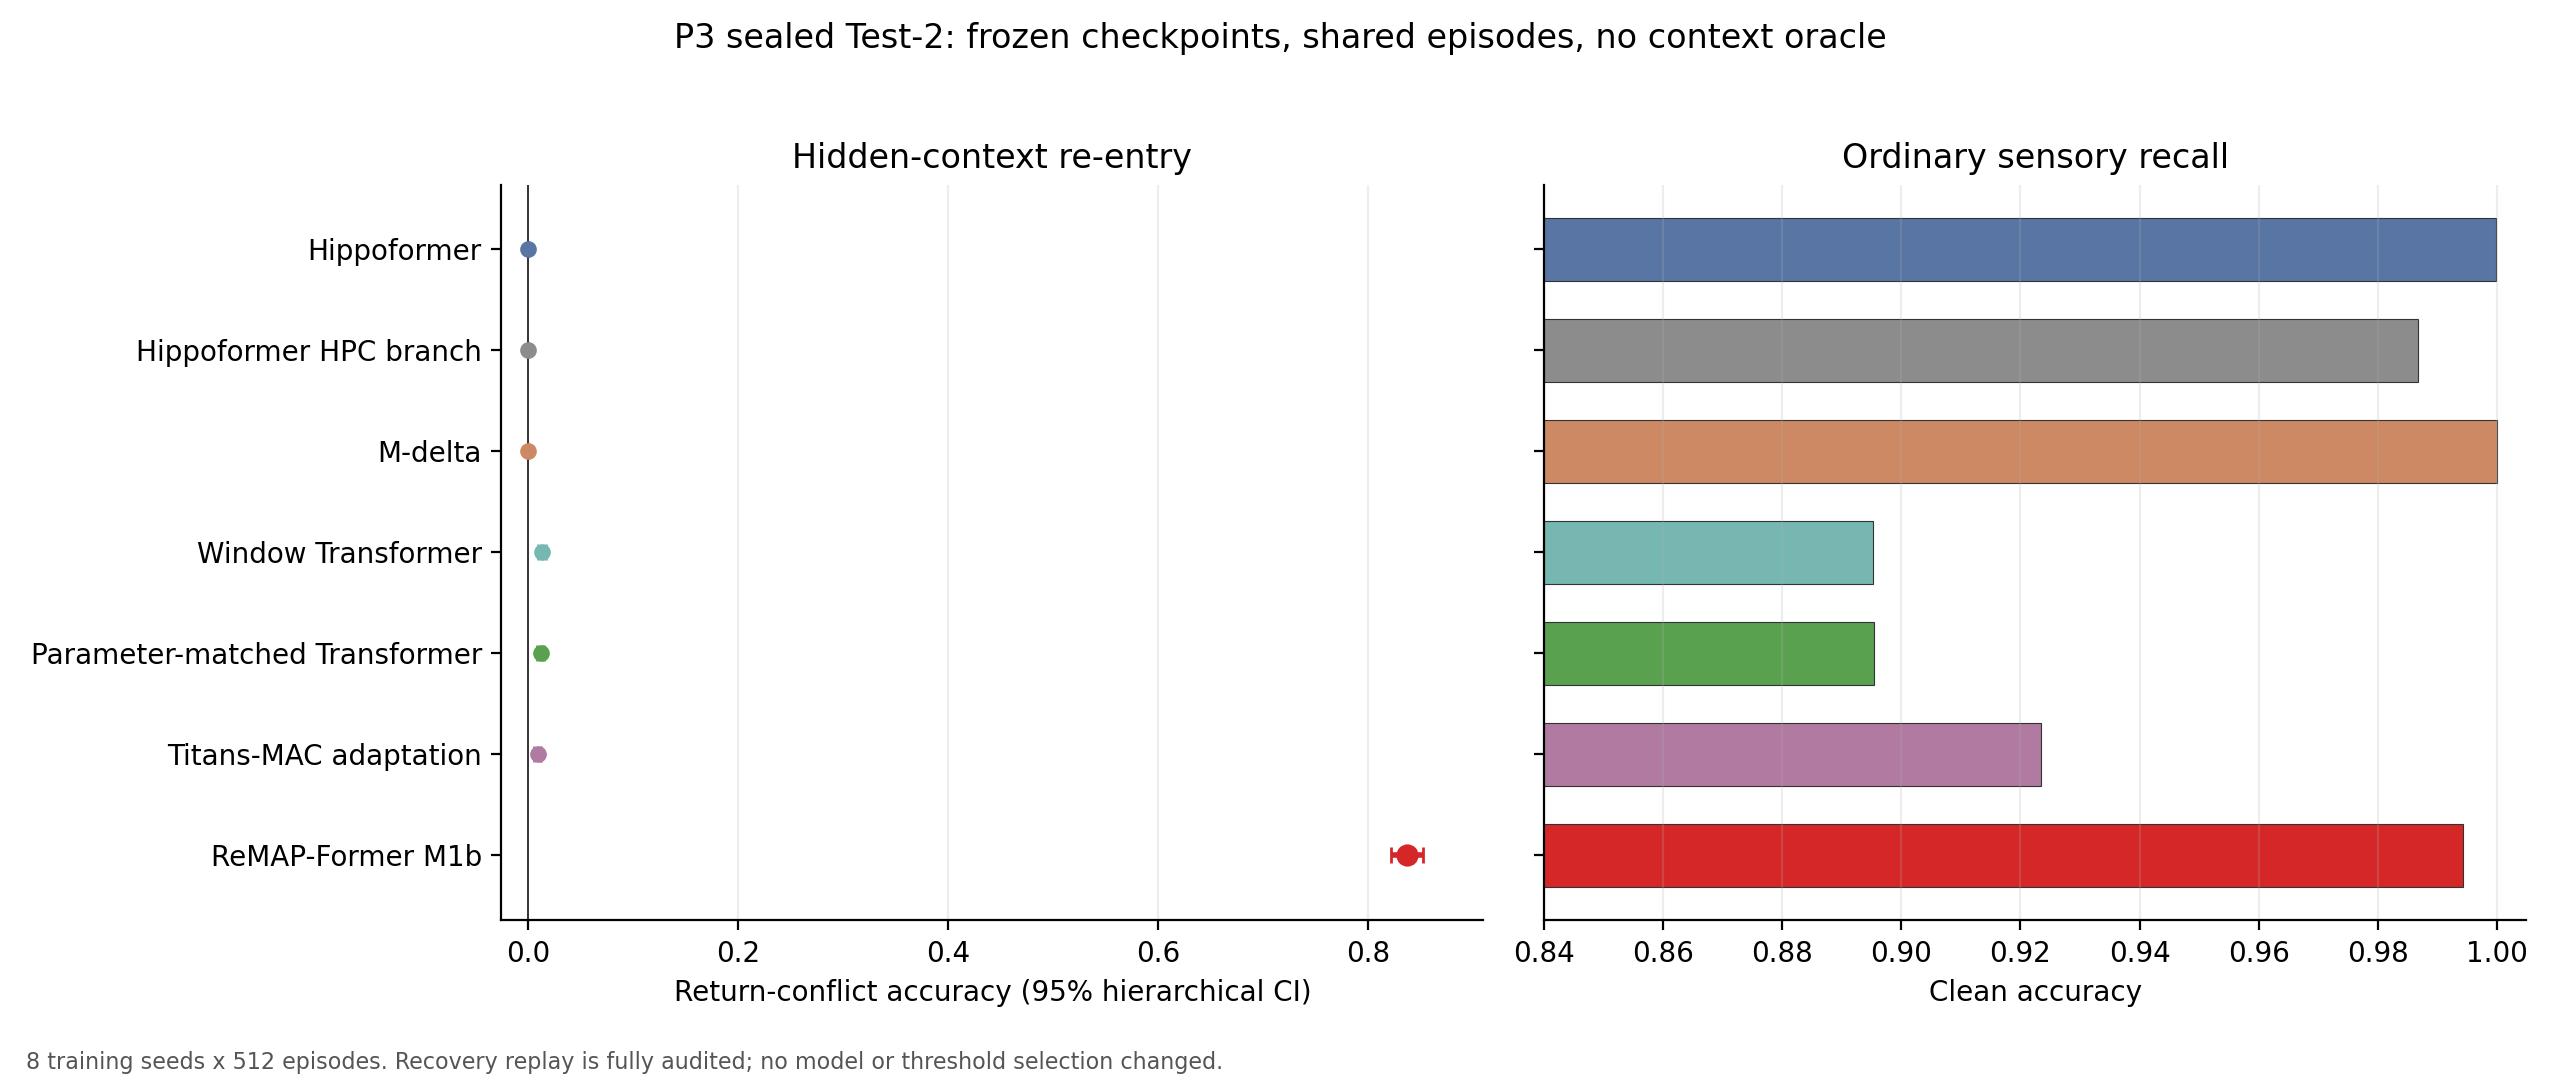
\includegraphics[width=0.96\textwidth]{remap_former_p3_test2.png}
\caption{P3 sealed Test-2。左：hidden-context return-conflict；右：ordinary clean recall。M1b 的优势集中在旧情境恢复，而 clean 几乎不受损。}
\label{fig:p3}
\end{figure}

\subsection{8-seed 稳定性与因果必要性}

8 个训练 seed 上，M1b return-conflict 为 $0.8201\pm0.0200$，范围 $[0.7852,0.8457]$；\base{} 与 \mdelta{} 均为 0。M1b clean 为 $0.9949\pm0.0019$。全部预注册稳定性门通过。

\begin{table}[H]
\centering
\small
\caption{8-seed component ablation。每个干预只用于定位机制。}
\begin{tabularx}{\textwidth}{YrrY}
\toprule
条件 & Return & 相对 Full & 判断\\
\midrule
\textbf{Full M1b} & \textbf{0.7944} & -- & 完整机制\\
No covariance correction & 0.2676 & -0.5268 & 去串扰更新必要\\
Fixed context & 0.0000 & -0.7944 & 历史 context 必要\\
Shuffled context & 0.4355 & -0.3589 & 正确 context 对齐必要\\
HPC zero & 0.0234 & -0.7710 & 外挂内容必要\\
Forced wrong return context & 0.0010 & -0.7934 & 错误重映射摧毁回忆\\
Correct-context oracle & 0.9424 & +0.1480 & 剩余上限主要在 context inference\\
\bottomrule
\end{tabularx}
\end{table}

该消融链排除了 ``只是更大的 Transformer''、``只是一个固定 fast-weight 分支'' 与 ``context 没有真正进入地址'' 三种解释。

\subsection{延迟、容量与边界}

Observed-history 长延迟在 8 seeds、长度 836 时保持 $0.8496\pm0.0246$；3 seeds、长度 4356 时为 0.7500。该实验每步仍观察真实历史，不是 strict free rollout。

\begin{table}[H]
\centering
\small
\caption{Novel-event capacity。Oracle 仅用于定位瓶颈。K50 是准确率仍高于 0.5 的最大 K。}
\begin{tabular}{lrrrrrrr}
\toprule
条件 & K1 & K2 & K4 & K8 & K12 & AUC & K50\\
\midrule
M1b normal & 0.776 & 0.711 & 0.375 & 0.193 & 0.099 & 0.462 & 4\\
Correct-context oracle & 0.982 & 0.948 & 0.672 & 0.388 & 0.206 & 0.691 & 8\\
Exact-address diagnostic & 0.987 & 0.971 & 0.836 & 0.737 & 0.477 & 0.844 & 12\\
\bottomrule
\end{tabular}
\end{table}

当前 2D 不支持 ``完整 strict rollout 曲线全面获胜''。预注册 full-curve H1 未通过，M1b-\base{} log-horizon AUC difference 为负；但 4096 endpoint difference 为 $+0.3688\,[0.2289,0.4836]$。官方 mm-TEM 的 64-step 结果尚未在本仓库忠实复现，不能把内部 branch 当成官方数字。

\section{3D Variable-Layout Visual Rollout}

\subsection{任务、baseline 与预算边界}

3D 模型根据动作与上一 RGB frame，在 strict free rollout 中递归生成未来视觉。未来 GT 不回灌。pixel MSE 越低越好。C20-H44 adaptive dev 的 best rollout MSE 如表~\ref{tab:3dbase}；所有外部 baseline 经 1200 rollout steps 后改善，但 M1b reference 继承约 12,180 ancestor updates，故该表只证明 catch-up 成功，不证明公平胜出。

\begin{table}[H]
\centering
\small
\caption{3D adaptive dev baseline catch-up。不是 sealed test，也不是 budget-matched 主表。}
\label{tab:3dbase}
\begin{tabularx}{0.82\textwidth}{Yrr}
\toprule
模型 & Best rollout MSE & Rollout 训练\\
\midrule
Transformer & 0.022994 & 1,200 steps\\
Titans adaptation & 0.021891 & 1,200 steps\\
\base{} adaptation & 0.023302 & 1,200 steps\\
M1b reference & \textbf{0.020073} & $\sim$12,180 ancestor updates\\
\bottomrule
\end{tabularx}
\end{table}

Open-9 写入策略中，full write MSE 为 0.029933，fixed K16 为 0.027157，改善 $9.28\%$。三 seed neural write gate 为 $0.027839\pm0.000682$：相对 full write 约好 $7\%$，但仍比简单 K16 差 $2.51\%$。稳定现象是 ``早写晚停''，而不是 learned writer 已经胜出。

\subsection{C3：当前冻结 3D 核心}

C3 将 visual content bottleneck 提升到 128D。variable-content gate 的 direct reconstruction error ratio 为 0.183588，actual retrieval error ratio 为 0.242422，retrieval cosine 为 0.918，证明 HPC 中的内容既可编码也可经实际地址取回。

\begin{table}[H]
\centering
\small
\caption{Validation episodes [224,288) 的 paired strict rollout。}
\begin{tabular}{lrr}
\toprule
条件 & Mean pixel MSE & 相对 PFC-only\\
\midrule
PFC-only & 0.01644746 & --\\
\textbf{C3 full} & \textbf{0.01593798} & \textbf{+3.0976\%}\\
\bottomrule
\end{tabular}
\end{table}

90\% paired bootstrap CI 为 $[-0.4999,+1.4387]\times10^{-3}$，跨零；44 个 horizon 中 37 个为正，但 p10 episode 仍存在负尾。因此 C3 是当前最干净的机制核心，而不是统计显著的最终 winner。

\begin{figure}[H]
\centering
\includegraphics[width=0.97\textwidth]{memorymaze3d_c3_variable_component_audit.png}
\caption{C3 variable-layout component audit。多数 horizon 上 full 低于 PFC-only，但平均改善较小且存在 episode 负尾。}
\label{fig:c3}
\end{figure}

\subsection{C4-C6：调用实验与正式负结果}

\begin{table}[H]
\centering
\small
\caption{调用与负尾机制链。所有失败版本均不替代 C3。}
\begin{tabularx}{\textwidth}{p{0.13\textwidth}Yp{0.23\textwidth}}
\toprule
版本 & 关键结果 & 决策\\
\midrule
C4 & 相对 C3 仅约 $+0.272\%$ & 不升级\\
C5 soft & Val [416,480)：0.01183695 vs PFC 0.01204335，改善 $1.7138\%$，CI 跨零 & 不升级\\
C5 hard & 改善 $0.4875\%$；p10 repair 为 $62-88\%$ & 负尾诊断\\
C6 G0 & held AUC 0.6159，BAcc 0.6019 & 允许进入 formal\\
\textbf{C6 formal} & \textbf{held AUC 0.5131，BAcc 0.4980} & \bad{\textbf{fresh blind 前停止}}\\
\bottomrule
\end{tabularx}
\end{table}

C6 在同一冻结 C5 生成历史上强制候选步 $\alpha_t=0$ 与 $\alpha_t=1$，用当前及未来最多 4 步的 detached RGB regret 生成 teacher；只训练原有 gate head。正式 fit AUC 为 0.9986，而 held AUC 为 0.5131；horizon-only 控制达到 0.5974。非 head 权重最大变化为 0，未来 target 改写不改变 gate features。

\begin{figure}[H]
\centering

\includegraphics[width=0.96\textwidth]{memorymaze3d_rollout_call_teacher_c6.png}
\caption{C6 formal。左：调用的未来收益呈明显时间结构，早期平均有利、后期平均有害。右：held 分类接近 chance，现有瞬时 features 未学到可跨 episode 泛化的 caller。}
\label{fig:c6}
\end{figure}

按预注册协议，C6 未生成新地图、未访问 fresh blind，不继续搜索 threshold、margin、loss 或 hidden size。该负结果定位的是 invocation 泛化失败，而不是 HPC 内容无效。

\section{证据等级与论文边界}

\begin{table}[H]
\centering
\small
\caption{截至 2026-07-25 的 claim ledger。}
\begin{tabularx}{\textwidth}{Yp{0.19\textwidth}Y}
\toprule
命题 & 等级 & 直接依据\\
\midrule
2D hidden-context re-entry 可行 & \good{\textbf{强}} & sealed test、8 seeds、因果消融\\
2D 长 observed-history 保持 & \good{\textbf{中强}} & 8 seeds 到 836，3 seeds 到 4356\\
2D 完整 strict free rollout 胜出 & \bad{\textbf{未成立}} & full-curve/AUC 不支持全面胜出\\
3D HPC content 可存可取 & \good{\textbf{强机制证据}} & 128D content/retrieval gate\\
3D full 优于 PFC-only & \caution{\textbf{趋势}} & $+3.10\%$，CI 跨零\\
3D learned write gate 优于 K16 & \bad{\textbf{未成立}} & 仍差 $2.51\%$\\
3D learned caller 可泛化 & \bad{\textbf{否定}} & C6 formal held AUC 0.513\\
3D 公平击败外部 baseline & \caution{\textbf{未检验完成}} & 训练预算与 cache 不匹配\\
\bottomrule
\end{tabularx}
\end{table}

当前最小可辩护贡献由四部分组成：(i) 无 oracle 的 PFC-EC-HPC 接口；(ii) 2D A-B-A re-entry 的跨 seed 正结果；(iii) 3D content capacity 与 C3-C6 调用边界；(iv) read-before-write、target-independence、metadata-independence、checkpoint-freeze 与 pre-blind stop 审计。当前不应使用 ``解决长期 free rollout''、``全面击败 \base{}/mm-TEM/Titans''、``learned caller 自动决定何时调用'' 或 ``3D 结果统计显著'' 等标题级措辞。

\section{下一阶段预注册路线图}

\subsection{P0：发布完整性}

旧 P5 release audit 发现归档中的 \texttt{remap\_former/pfc.py} hash mismatch。任何新 sealed test 前必须从当前 source、协议、checkpoint、summary 与 figure 重建 canonical release，固定环境、命令、seed 和 split hash，并保持 76/76 tests。

\textbf{Go gate：}clean checkout 可一键重跑评估并匹配全部冻结 summary；任何 hash mismatch 都停止 sealed test。

\subsection{P1：2D strict free-rollout headline}

在 horizons $\{2,4,8,16,32,64,128,256,512,1024,2048,4096\}$ 上运行 8 paired seeds，报告 accuracy、log-horizon AUC、4096 endpoint、clean 与 return-conflict。observed-history 与 strict free rollout 分表。所有 baseline 使用相同训练/evaluation budget；mm-TEM 只有在忠实复现官方 64-step protocol 后进入正文。

\textbf{Go gate：}M1b 的 return-conflict 优势保持，且 strict curve 的预注册主指标至少一个显著优于 \base{}。否则 headline 只保留 re-entry，不宣称 rollout superiority。

\subsection{P2：3D 公平预算与 fresh blind}

冻结 C3，不加入新 gate。为 \base{} 实现 incremental rollout cache 并做逐步等价测试；按 optimizer steps、seen frames、参数量与 wall-clock 分层比较 Transformer、Titans adaptation、\base{} 与 C3。development 至少 3 seeds，最终 5-8 seeds；fresh layout hashes 与所有已见 manifest 严格不相交，sealed blind 只打开一次。

\textbf{Go gate：}C3-PFC 的 95\% paired CI 不跨零，且在公平预算下相对至少一个 strongest external baseline 保持优势。否则 3D 只作为机制扩展。

\subsection{P3：2D 到 3D 的 hidden-context bridge}

在同一几何位置的不同视觉 context 中绑定不同内容，构造 A-B-A route re-entry；入口与路径族跨 split。模型仍不读取 room、context、pose 或 switch。任务 gate 要求 trajectory-history room probe 高、cue-only 接近 chance、真实歧义率充分。

\textbf{Go gate：}full 在 re-entry 上显著优于 PFC-only 与 fixed-context，wrong-context/HPC-zero/no-covariance 产生结构化退化，clean drop 不超过 2 pp。

\subsection{P4：容量与尺度律}

正交改变 content dim $\{64,128,256\}$、place sparsity、novel events $K\in\{1,2,4,8,12,16\}$、maze size、horizon 与 context 数量；报告 direct/retrieval ratio、cosine、K50、MSE、计算量与显存。

\textbf{Go gate：}出现跨 seed 稳定的容量规律，而不是单 checkpoint 改善。

\subsection{P5：caller 重开条件}

C6 后暂停瞬时 gate 调参。只有具备 recurrent uncertainty state、多个独立 teacher pools、预先冻结的容量/正则/early-stop，并继续禁止 age/K token、位置、room/context 标签与第二套记忆时才重开。

\textbf{Go gate：}held AUC $\geq0.60$、BAcc $\geq0.55$，且 AUC 同时比 source 与 horizon-only 高至少 0.02。未通过则保持 C3 static invocation。

\begin{table}[H]
\centering
\small
\caption{推荐执行顺序。并行只保留 baseline cache 工程，避免同时扩散模型线。}
\begin{tabularx}{\textwidth}{p{0.10\textwidth}Yp{0.20\textwidth}}
\toprule
顺序 & 工作 & 论文作用\\
\midrule
1 & P0 release integrity & 封死证据链\\
2 & P1 2D strict curve & 最接近 headline\\
3 & P2 3D fair blind & 把趋势升级为证据\\
4 & P3 visual hidden-context & 统一 2D/3D 课题\\
5 & P4 scale law & 租卡阶段批量运行\\
暂停 & P5 caller & 等待新状态设计\\
\bottomrule
\end{tabularx}
\end{table}

\section{结论}

\model{} 当前不是一个 ``所有 rollout 都赢'' 的完成品，而是一条已经有清晰核心与清晰边界的研究线。2D 结果说明：当 Transformer/PFC 必须从历史推断 context 时，context-dependent address 与 episode-local HPC 能恢复普通窗口模型、\base{} 和单映射 delta memory 无法恢复的旧内容。3D 结果说明：同一 neural HPC 可以进入视觉自由滚动并产生可测的内容收益，但简单写入预算、episode 负尾和 caller 泛化仍是主要瓶颈。最有价值的下一步不是继续堆 gate，而是完成 release integrity、严格 rollout 主曲线、公平 3D blind test 与视觉 hidden-context bridge。

\begingroup
\footnotesize
\setlength{\bibsep}{1pt}
\bibliographystyle{iclr2025_conference}
\bibliography{remap_former_iclr_design}
\endgroup

\end{document}
